\documentclass[12pt]{report}
\usepackage{graphicx,amssymb,amsmath,amsthm,ctable,booktabs,graphics}
\usepackage[colorlinks]{hyperref}
\usepackage[all]{hypcap} 
\usepackage{gensymb}
\usepackage{xcolor}
\usepackage{savetrees}
%\renewcommand{\familydefault}{\sfdefault}
\usepackage[english]{babel}
%\usepackage[T1]{fontenc}
%\usepackage{helvet}
\usepackage{multicol}
\usepackage[utf8x]{inputenc}

\newcommand{\ty}[1]{\textcolor{teal}{\texttt{#1}}}
\begin{document}

\title{Gemini-South IFU Data Reduction User Manual}
\author{Elaine M. Snyder\\
Dept. of Physics \& Astronomy\\
University of North Carolina at Chapel Hill \\
\texttt{emsnyder@live.unc.edu}}
\date{February 22, 2016}
\maketitle

\hypersetup{linkcolor=magenta}
\tableofcontents
\listoftables
\listoffigures

%\begin{multicols*}{2}

\chapter{Introduction}
Greetings, Gemini Multi-Object Spectrograph (GMOS) integral field unit (IFU) data reduction pipeline user! Before beginning your data reduction journey, it will be important to understand the structure of an IFU and the way the Gemini IFU data is stored. If you are familiar with this already, feel free to skip ahead. Most of this information can be found online on \url{https://www.gemini.edu}, but I've compiled it all here for easy reference and so that I may reference it in the context of the RESOLVE\footnote{\url{http://www.resolve.astro.unc.edu}} survey's instrument setups.

The basic idea of any IFU is that you obtain multiple spectra over the face of a galaxy, instead of getting one spectrum as you would using a long slit, which enables spatial analysis of the kinematics/metallicities/whatever you want to get out of your spectra. In the case of the GMOS IFU setups for RESOLVE observations, you will have either 750 or 1500 fibers that cover a region on the sky $5''\times3.5''$ or $7''\times5''$ (each fiber covers $0.2''$). The GMOS IFU is designed in such a way that not all of those fibers are centered on the object. Either 250 or 500 of the fibers are positioned on a region of sky away from the target (but not too far away), which enables the sky level to be later subtracted during data reduction (you will do this soon!). The sky level can be affected by moon illumination, clouds, etc. so it is important to be able to subtract any extra sky light there may be. Note that sometimes in online documents, the fibers may be called ``spaxels'', which is short for ``spectral pixels'' -- don't be confused by this hip IFU lingo. The top portion of \autoref{figure:1} shows the positions of the fibers over an example galaxy.

\begin{figure}[h]
\centering
\includegraphics[width=0.8\textwidth]{fiber_examples.jpeg}
\label{figure:1}
\caption[IFU Fibers and Data Format]{The top part of this image shows the IFU field of view over NGC221 (not a part of RESOLVE). The left portion of the image shows the sky spaxels, and the right portion shows the light of the galaxy. This is a 2D representation of the data we are getting -- the third dimension is in the wavelength direction, and the darkness over where the galaxy is from summing the light inside each spaxel there. The bottom portion of this image shows the raw fits data from the above galaxies.  \footnotesize{Image from \url{https://www.gemini.edu/sciops/instruments/gmos/spectroscopy/integral-field-spectroscopy/field-slit-mapping}}}
\end{figure}

\section{Observing Setups}
There are two main setups for RESOLVE's IFU observations. Similarly to our SOAR observations, there is a blue setup for absorption line galaxies and red setup for emission line galaxies. \autoref{table:1} highlights the main differences in the two setups. To determine which galaxy is best for which setup, we ideally like to use the SOAR broad spectrum as a guide. Seeing strong emission in the broad spectrum will point to the emission line setup on Gemini being best, while no emission will point to the absorption line setup being preferred. However, since there is not always a SOAR (or even SDSS) spectrum available, we often rely on their photometric colors as an indicator of whether emission or absorption is more likely.

We estimate exposure times for both setups using the online Integration Time Calculators\footnote{\url{http://www.gemini.edu/node/10479}} (ITC). We use an elliptical galaxy SED template for estimates in the blue setup, and the H$\alpha$ line with an estimate of the line flux and continuum flux density for estimates in the red setup. We bin all our spectra by 2 spectrally to increase the signal-to-noise. For the blue setup, we set our exposure time calculations to achieve signal-to-noise 25 per \AA\ when we bin all the fibers out to the effective radius of the galaxy. For the red setup, we set up our exposure times to achieve a centroiding accuracy of $\sim5.3$ km s$^{-1}$.

We also use the ITC to select central wavelength positions that ensure our features of interest do not fall in a chip gap (see bottom of \autoref{figure:1}).  

\begin{table}
\centering
\begin{tabular}[t]{ccc}
  \hline
quantity  & blue setup & red setup \\ \hline
wavelength range & 4200 -- 5600 \AA\ &  5500 -- 6900 \AA\ \\ 
used for & absorption line galaxies & emission line galaxies \\ 
features of interest & H$\beta$, Mgb, Fe5270, Fe5335 & H$\alpha$, [NII], NaD \\ 
grating & B1200 & B600 \\ 
filter & none & r-G0326 \\
slits & 1 slit & 2 slits \\ 
field of view & $3.5''\times5''$ & $5''\times7''$ \\ \hline
\end{tabular}
\caption[RESOLVE's Observation Setups]{Comparison of RESOLVE's red and blue observation setups for the Gemini-South IFU.}
\label{table:1}
\end{table}

\section{Observing Patterns}
In 2-slit, aka red setup, mode, we oftentimes will tile the IFU field of view in order to cover the entire extent of the galaxy. The $5''\times7''$ field of view can either be tiled to $10''\times7''$ for larger, rounder galaxies or to  $5''\times14''$ for longer, skinnier galaxies. This doesn't make a large difference to the reduction routine, but there will be more science frames to reduce and more data cubes to stack at the end.

The basic observation sequence is different for each mode. Both will start with acquisition images to ensure the IFU field of view is centered on the galaxy. Then flats, arcs, and science frames are taken in each central wavelength position together. For example, 

\section{How the Gemini Data is Stored}
Why 12 extensions?
What is an MDF file?



\chapter{Setting Up Your Workspace}

There are some things you'll need to install (or update) before using this pipeline. I highly recommend working in the Ureka environment, which includes easy-to-install versions of IRAF, Python, and Pyraf. Since this code is written for Pyraf, Ureka is indeed quite handy. Instructions on how to download Ureka can be found here: \url{http://ssb.stsci.edu/ureka/}. I am currently using version 1.5.1 on cielo. Follow the instructions for making IRAF, and check your login screen to make sure it says you're using IRAF 2.16:

\begin{verbatim}
NOAO/IRAF PC-IRAF Revision 2.16 EXPORT Thu May 24 15:41:17 MST 2012
  This is the EXPORT version of IRAF V2.16 supporting PC systems.
\end{verbatim}

There is also an updated IRAF Gemini package you'll want to install. This version is not included in the Ureka download, but includes some updated tasks you will be using. Here's the link to this newest version as of February 2016: \url{https://www.gemini.edu/?q=node/11823}. You'll also want to check this when you're done by loading the `gemini' package in IRAF:

\begin{verbatim}
--> gemini

     +------------------- Gemini IRAF Package -------------------+
     |             Version 1.13.1, December 7, 2015              |
     |             Requires IRAF v2.14.1 or greater              |
     |              Tested with Ureka IRAF v2.16                 |
     |             Gemini Observatory, Hilo, Hawaii              |
     |    Please use the help desk for submission of questions   |
     |  http://www.gemini.edu/sciops/helpdesk/helpdeskIndex.html |
     +-----------------------------------------------------------+
\end{verbatim}


If you are new to data reduction in general, you will want to download ds9, an astronomical imaging application that you'll use to view our data as you progess through the pipeline. Download ds9 from this site: \url{http://ds9.si.edu/site/Home.html}.

Next, you'll want data to actually reduce! You should have flats, arcs, science frames, response flats (from the standard star data), and a bias image before getting started. There should also be an observing log to inspect (RESOLVE data has obslog.txt or just log.txt). Place all of these images in the same folder, since that's where the pipeline looks for them. 

Lastly, you'll want to download the actual pipeline. You can access the code and this handy user guide at \url{https://github.com/emsnyder/geminiDRpipeline}. Always be on the lookout for updates in the future! You can place the code anywhere you like, but a nice folder structure would be to have individual folders for each galaxy with the pipeline code a level above. Now you should be all set, congrats!

\chapter{Data Reduction Guide}

\section{Entering and Exiting the Pipeline}
Here are the basic start up commands: 
\begin{enumerate}
\item cd to the directory where you put your data
\item enter the Ureka environment by typing \ty{ur\_setup} in the command line 
\item enter PyRAF by typing \ty{pyraf} in the command line
\item open a ds9 window by typing \ty{!ds9 \&} at the prompt
\item enter the pipeline by typing \ty{execfile(`/path/to/your/code/gemreductionpipeline.py')}
\end{enumerate}

\noindent To end your session:
\begin{enumerate}
\item type \ty{CTRL-C} to exit the pipeline, if not out already
\item enter \ty{.exit} to exit PyRAF
\item use \ty{ur\_forget} to exit the Ureka environment
\end{enumerate}

\section{Organizing and Identifying Your Data}

\noindent The first thing the pipeline does is look in your folder and identify which files are there. It will print out the files it found and whether there are arcs/flats/science/etc. It is good to check this against your observing log! If you find mistakes, please email Elaine!

\section{Reduction of the Flats}

This very first step is often (in the author's experience) the most time-consuming and frustrating step of the entire reduction. We use the flats not only for flat fielding the science data, but also to identify all the fibers and use this identification as a reference for all the other files.

The program used here is a main part of the Gemini IRAF package called `gfreduce'. It has many different options, but for the flat, we are just going to do a bias subtraction, overscan subtraction, and fiber ID so that we may extract all the spectra.

\begin{enumerate}
\item The bias subtraction is done without user input needed. A file is produced in your working directory with the prefix `g'.
\item The overscan subtraction is mostly done without user input need. A PyRAF window does open, and you will step through each of the 12 image extensions (one for each CCD amplifier). There is a fit being plotting, and I normally just press \ty{q} inside the PyRAF window since the fit found looks fine. If the fit does not look fine, you can type \ty{:order \#} inside the PyRAF window to change the order of the fit to a different number (with that number instead of \# in the previous command). See Figure \ref{fig:overscan} for an example of what you should be seeing. This step produces a file with the prefix `rg', where the `g' comes from the previous step, i.e. the `rg' is both overscan and bias subtracted.
\item Lastly, we must tackle the fiber identification. Your command window is going to ask you a few questions:
\begin{verbatim}
Extracting slit 1
Find apertures for ergS20151108S0053_1? (`yes'): 
\end{verbatim}
Here I recommend saying `yes', as usually IRAF will be able to identify the fibers correctly for you. 
\begin{verbatim}
Edit apertures for ergS20151108S0053_1? (`yes'): 
\end{verbatim}
Say `yes' to this one as well, so we can inspect the fiber IDs and make sure everything looks correct. Figure \ref{fig:ap1} shows what this will look like -- a complete mess! But we can zoom in by typing \ty{w} in the PyRAF window, and then typing \ty{e} at the bottom-left of the first `fiber bundle' and again at its top-right. [Note: use \ty{w} and \ty{a} to un-zoom the window.] You should now have a screen that looks like Figure \ref{fig:ap2}. I find that making this plot full-screen helps immensely. Each `bundle' contains a set of 50 fibers, which you will see numbered at the top of your screen (though not very apparent in Figure \ref{fig:ap2}). Your job is to make sure each fiber is identified correctly -- this means no repeated numbers or missing fibers. Often I find that the low level of fiber 50 makes it get skipped in IRAF's auto-finding scheme, which makes the first fiber of the second `bundle' start at 50 instead of 51. If this happens, you can use \ty{d} in the plot window to delete the IDs for fibers 50--750, and then use \ty{m} to re-mark the fibers. This is where it can get frustrating! \\

Figure \ref{fig:bad} shows an example of a bad fiber not being marked in the identification process. This is exactly what we want to happen in this case. If you find another fiber that looks bad, you will have to edit the MDF file to `turn off' that fiber number. For the 2014-2015B slit-1 data, you will end with fiber 742 (743--750 are bad). If you're in the blue setup (1-slit mode), this is the end of IDing for you! If you're in the red setup (2-slit mode), you'll have to repeat this process for fibers 751--1500. \\


If you are pleased with your IDs, type \ty{q}. More questions will appear in the terminal, but it will want your answer inside the PyRAF graphics window.

\begin{verbatim}
Trace apertures for ergS20151108S0053_1? 
\end{verbatim}

\ty{yes}

\begin{verbatim}
Fit traced positions for ergS20151108S0053_1 interactively?
\end{verbatim}

\ty{NO} (the capitals will tell IRAF no to all)

\begin{verbatim}
Write apertures for ergS20151108S0053_1 to database
\end{verbatim}

\ty{yes}

\begin{verbatim}
Extract aperture spectra for ergS20151108S0053_1?
\end{verbatim}

\ty{yes}

\begin{verbatim}
Review extracted spectra from ergS20151108S0053_1?
\end{verbatim}

\ty{NO}

\end{enumerate}

\begin{figure}[h]
\centering
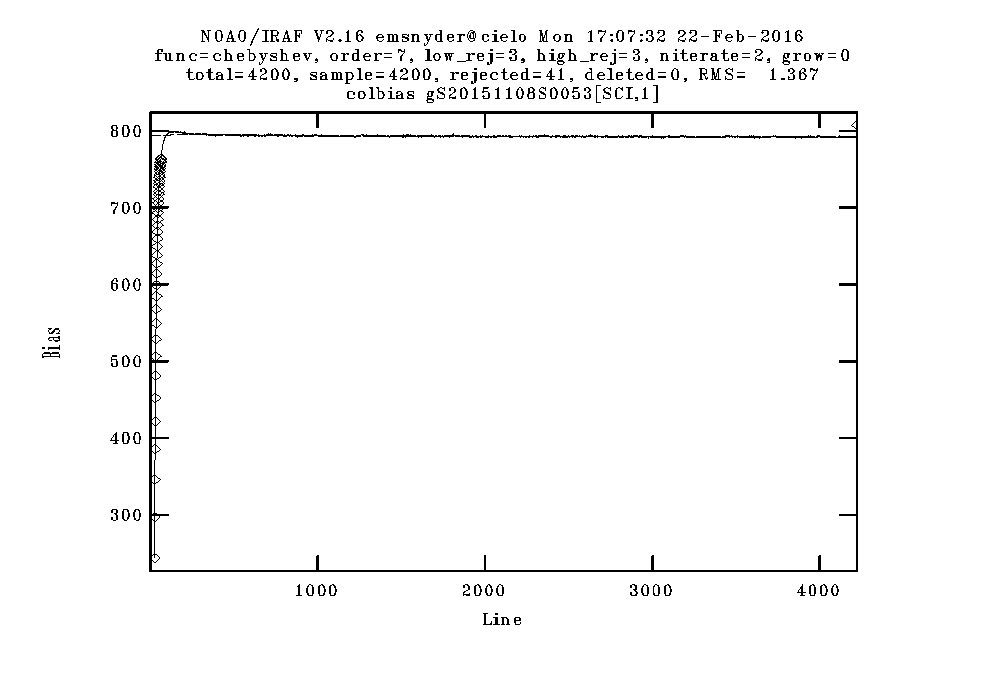
\includegraphics{overscan_example.eps}
\label{fig:overscan}
\caption[Overscan Subtraction Example]{An example of the overscan subtraction window that PyRaf will open during the reduction of the flats step. The solid line represents the data, while the dashed line shows the fit to that data. The diamonds are data points that are being rejected from our fit.}
\end{figure}

\begin{figure}[h]
\centering
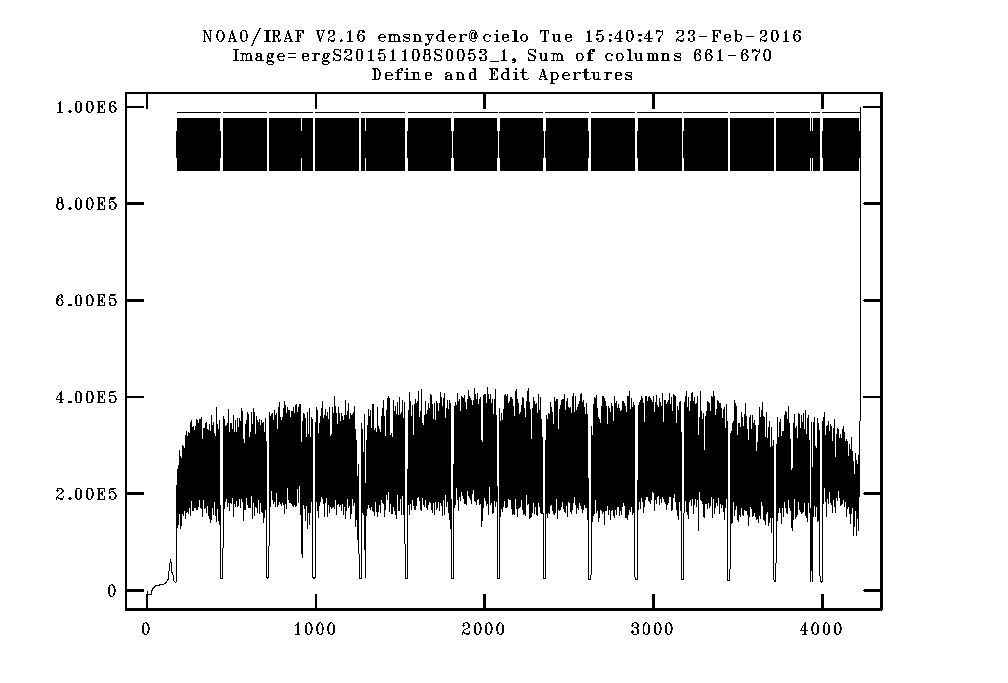
\includegraphics{apertures1.eps}
\label{fig:ap1}
\caption[Zoomed Out Fiber ID Example]{An example of the fiber ID window that PyRaf will open during the reduction of the flats step.}
\end{figure}

\begin{figure}[h]
\centering
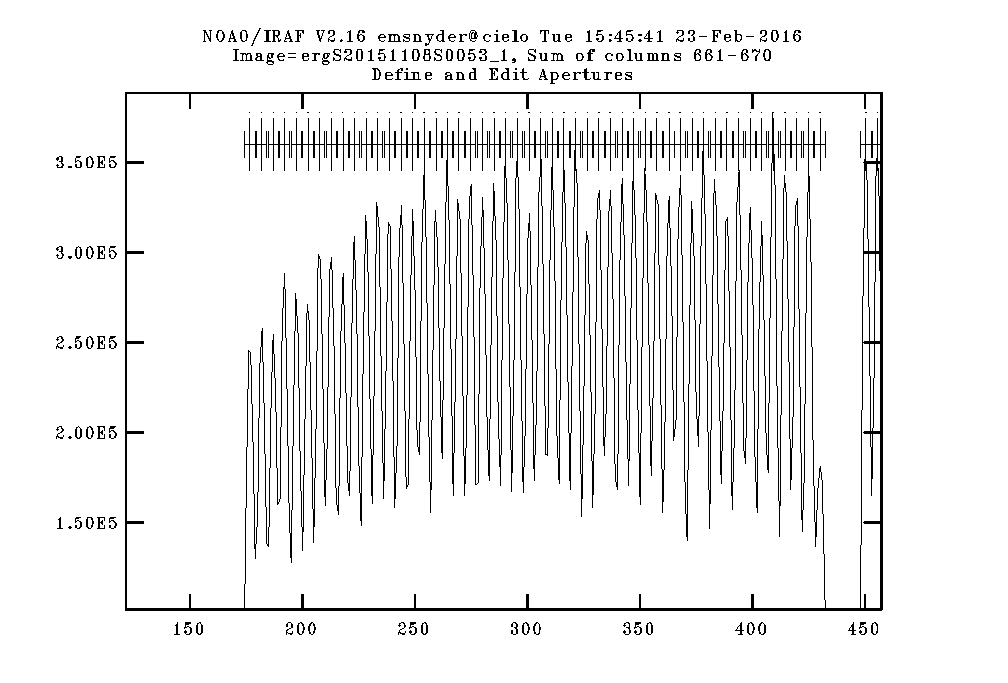
\includegraphics{apertures2.eps}
\label{fig:ap2}
\caption[Zoomed In Fiber ID Example]{An example of the fiber ID window that PyRaf will open during the reduction of the flats step.}
\end{figure}

\begin{figure}[h]
\centering
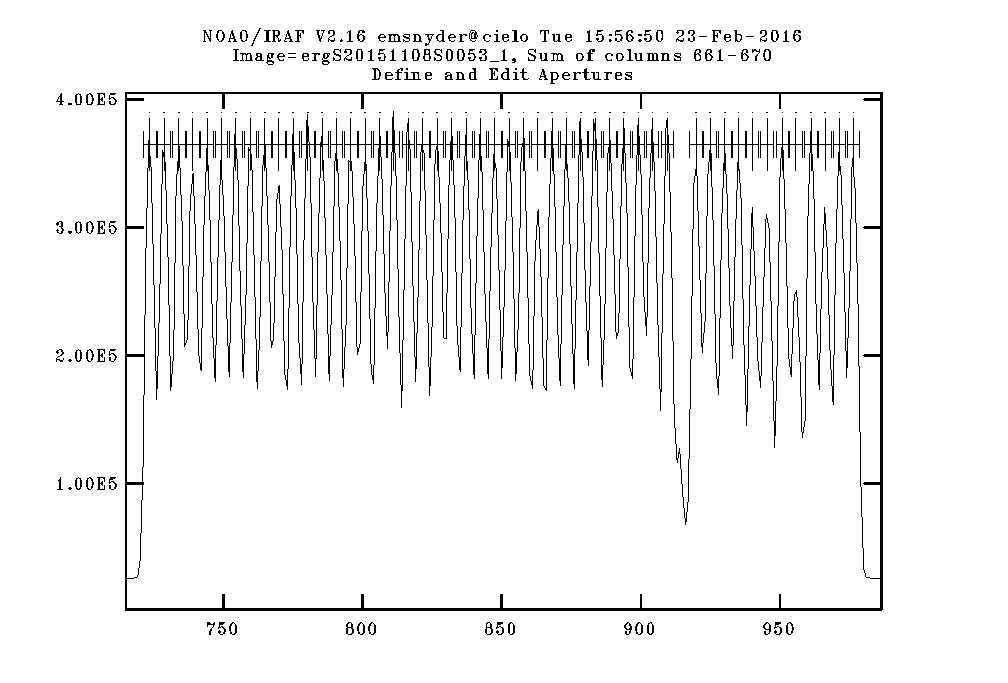
\includegraphics{badfiber.eps}
\label{fig:bad}
\caption[Example Image of a Bad Fiber]{For this image, fiber 138 is bad. The MDF knows this though, and that number is skipped during the identification routine.}
\end{figure}


\section{Reduction of the Arcs}

The next step is to overscan subtract the arcs. There is nothing interactive for this step.

\section{Wavelength Calibration of the Arcs}

This step is twofold: first we must find the wavelength solution for each arc lamp, and second, we must actually apply it to the arc as a check.

\subsection{Find the Wavelenth Calibration}


\subsection{Apply the Calibration to the Arcs}




\chapter{Derivation of Kinematics}

\section{Deriving Velocity Dispersions}
\section{Deriving Rotation Curves}

\chapter{Timeline of Pipeline Updates}


%\end{multicols*}


\end{document}
